\section{Конструкторский раздел}

\subsection{Метод распознавания суицидальных паттернов поведения человека по текстовым сообщениям}

Метод распознавания суицидальных паттернов поведения человека по текстовым сообщениям включает в себя xранение и анализ сообщений пользователей -- для определения, является ли сообщение суицидальным, используется модель машинного обучения. В качестве обучающей выборки используется дополненный датасет размеченных сообщений из открытого доступа \cite{dataset}.

\subsection{Формат и метод сбора данных }

В качестве задействованных в анализе данных используются текстовые сообщения и их даты написания, так как представленная зависимость количества смертей от суицида в зависимости от года и месяца говорит о возможной корреляции месяца написания сообщения и его возможной интерпретации.

Для сбора данных было задействовано автоматизированное средство сбора суицидальных сообщений в мессенджере Telegram. Интерфейс программного обеспечения позволяет направить в систему хранения два типа сообщений: суицидальные и на суицидальную тематику. 

Согласно 152-ФЗ ``О персональных данных'', ``персональные данные -- любая информация, относящаяся к прямо или косвенно определенному или определяемому физическому лицу (субъекту персональных данных)'' \cite{fzpers}. Таким образом, к персональным данным можно отнести фамилию, имя и отчество, дату и место рождения, адрес проживания, семейное, социальное и имущественное положение, образование, профессию, доходы и другое. В связи с этим средство сбора информации, не обрабатывает и не хранит никаких персональных данных о пользователях, направивших сообщения.

\subsection{Декомпозиция системы}

На рисунке \ref{img:useCase} представлена диаграмма вариантов использования системы.

\begin{figure}[H]
	\centering
	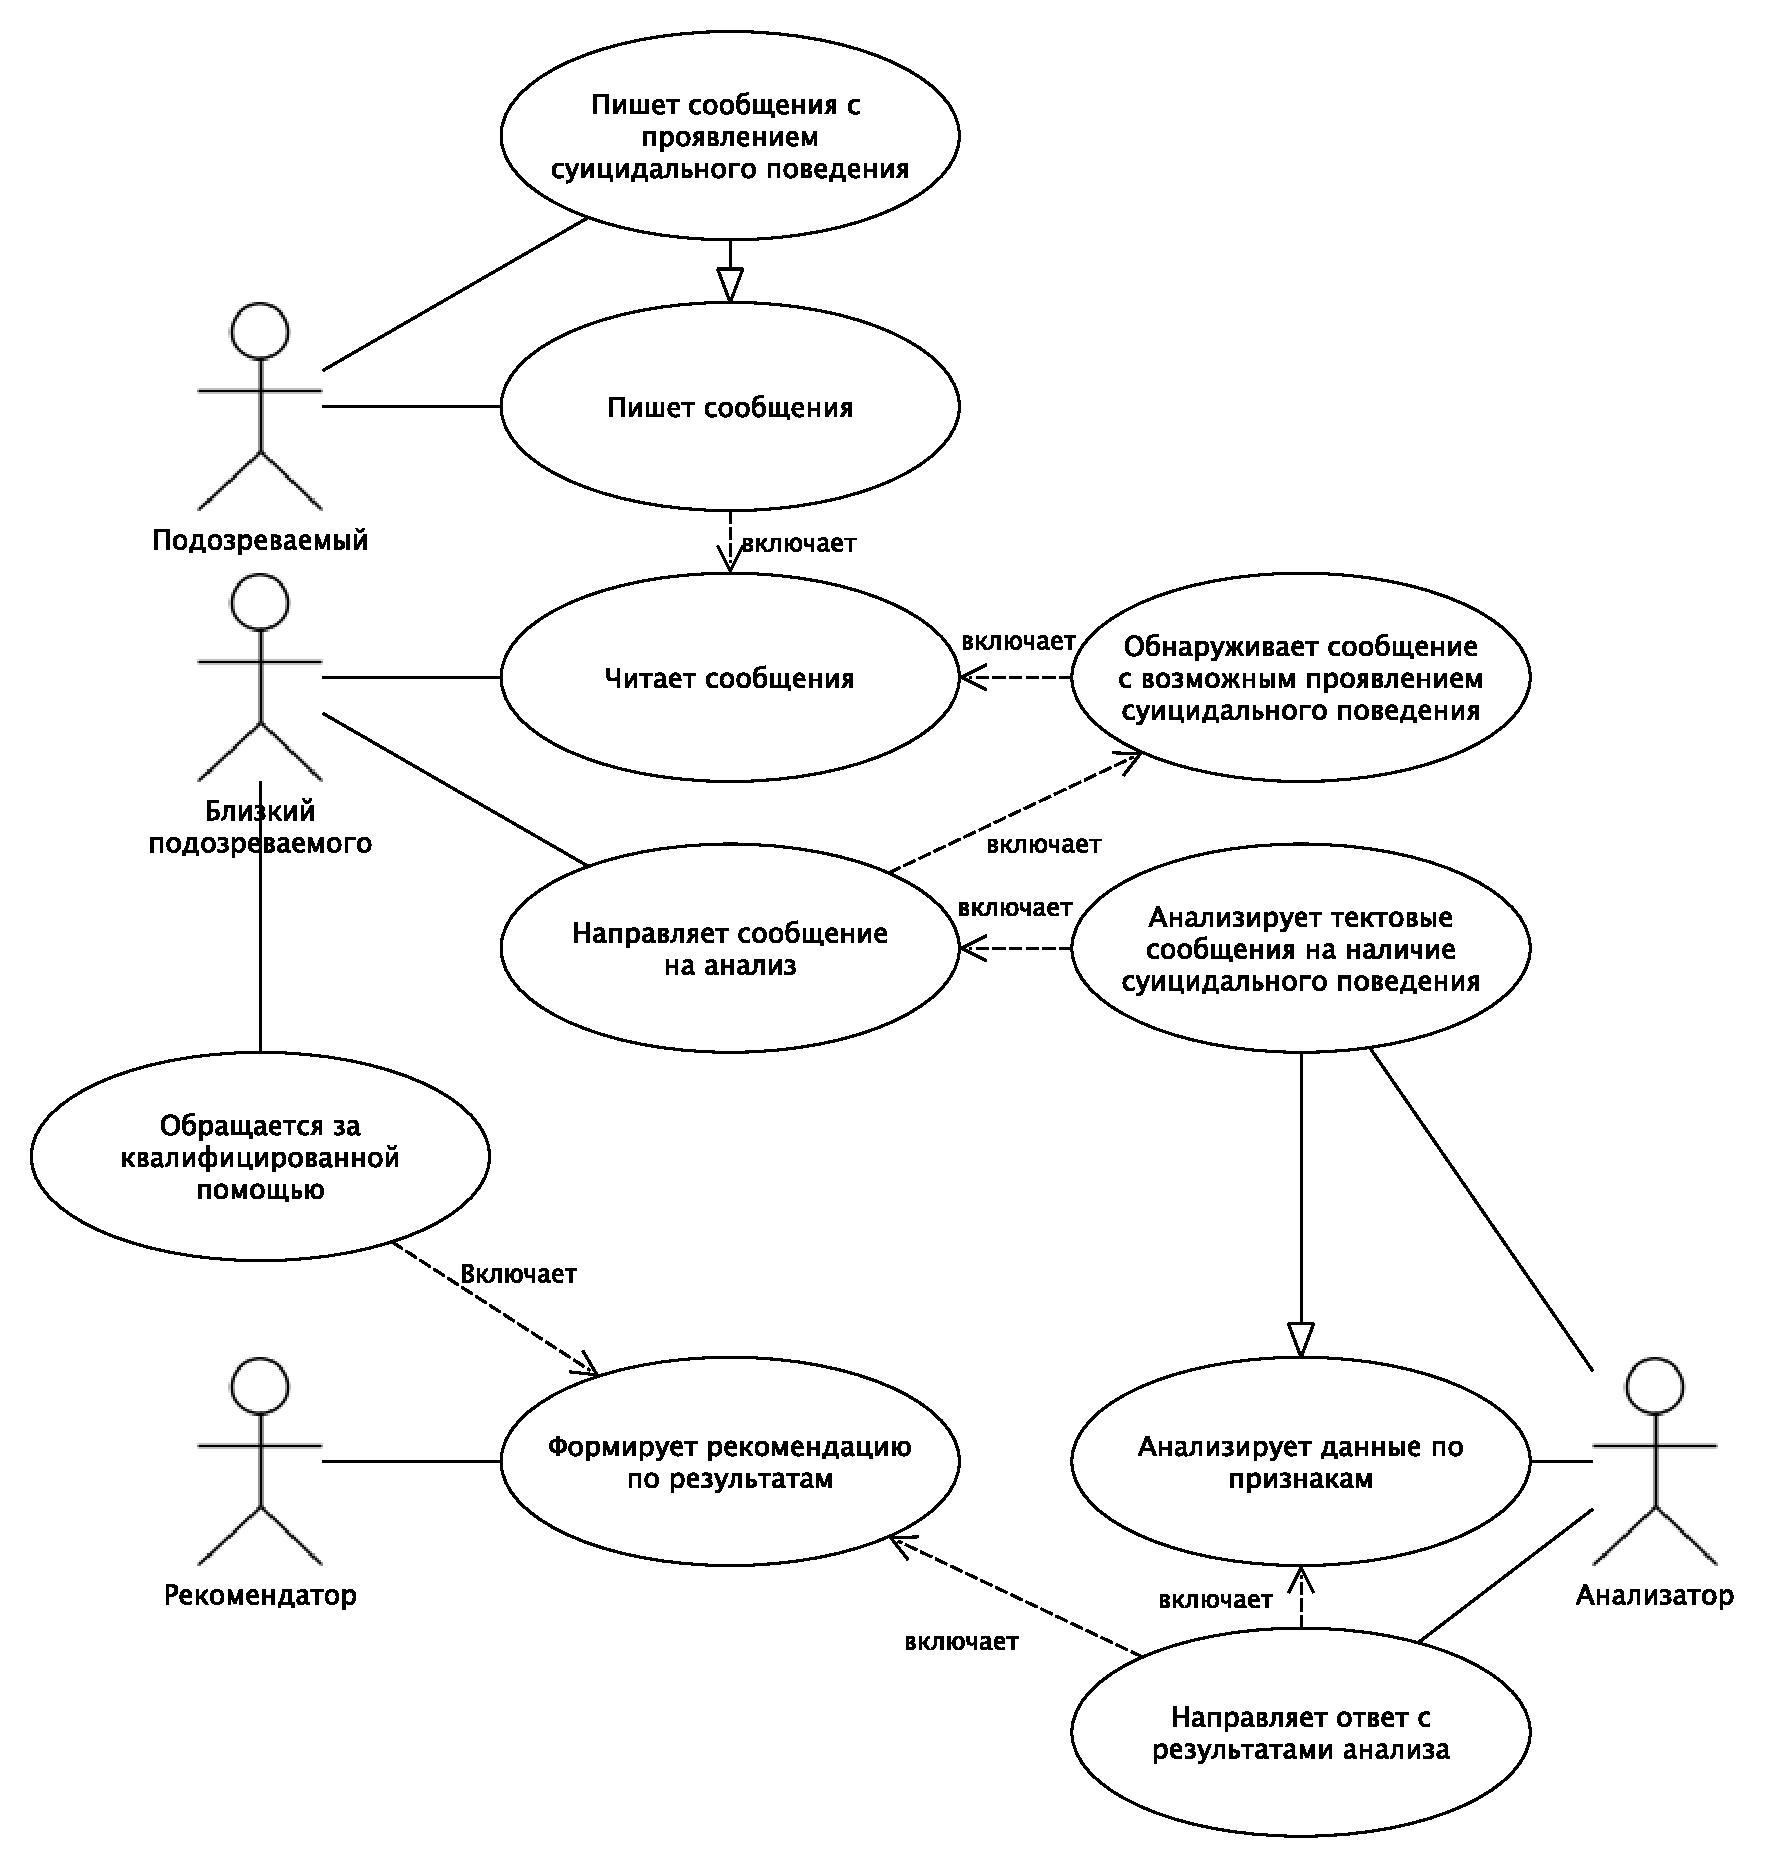
\includegraphics[width=\textwidth]{inc/useCase.pdf}
	\caption{ Диаграмма вариантов использования системы. }
	\label{img:useCase}
\end{figure}

На рисунках \ref{img:idef0}--\ref{img:idef1} представлены IDEF0 диаграммы задачи определения наличия суицидальных паттернов в текстовом сообщении.


\begin{figure}[H]
	\centering
	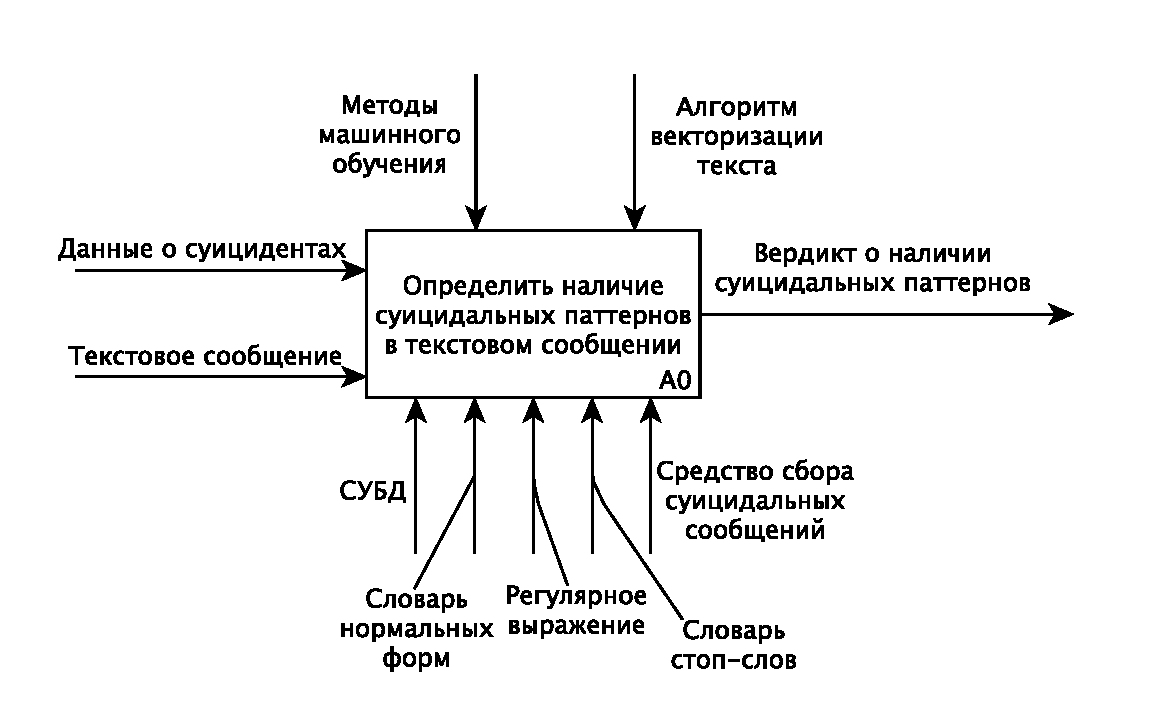
\includegraphics[width=\textwidth]{inc/A0.pdf}
	\caption{ IDEF0 диаграмма уровня А0. }
	\label{img:idef0}
\end{figure}

\begin{figure}[H]
	\centering
	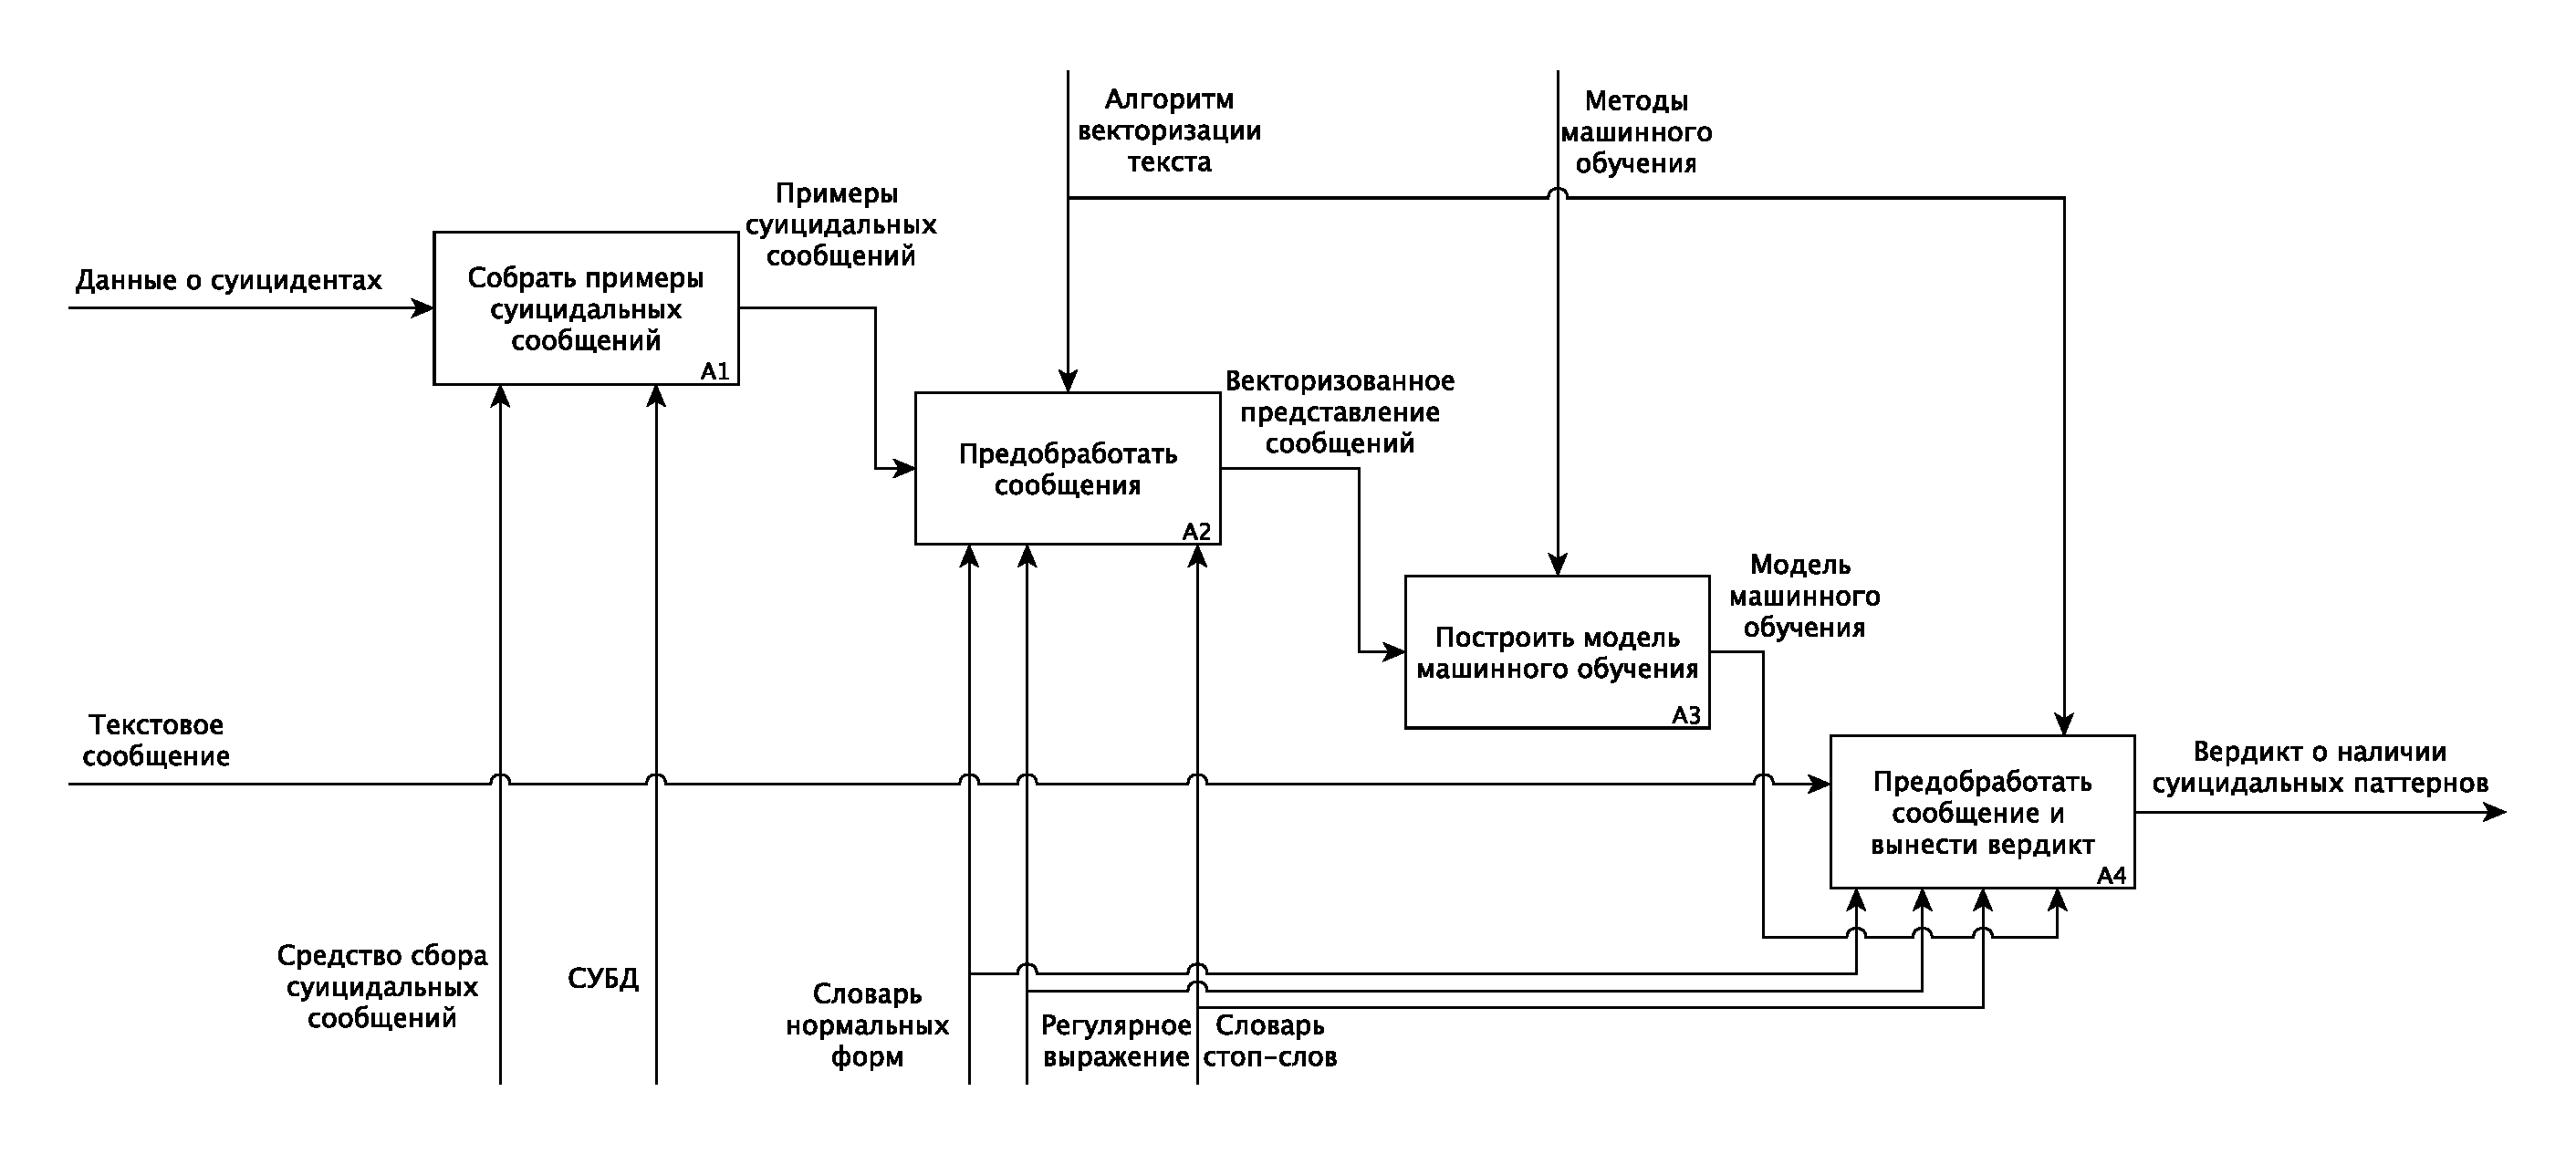
\includegraphics[width=\textwidth]{inc/A1.pdf}
	\caption{ IDEF0 диаграмма уровня А1-A3. }
	\label{img:idef1}
\end{figure}

\pagebreak